\section{Introducción}
En Sinatra 1.3 se introdujo el stream helper. 
El stream object imita a un objeto IO.

\begin{enumerate}
\item 
\htmladdnormallink{Código del método stream}{https://github.com/sinatra/sinatra/blob/master/lib/sinatra/base.rb\#L427-L437}
\item 
\htmladdnormallink{Class Stream code}{https://github.com/sinatra/sinatra/blob/master/lib/sinatra/base.rb\#L383-L425}: Class of the response body in case you use \verb|#stream|
\end{enumerate}

En ocasiones queremos empezar a enviar datos mientras se esta generando aún el cuerpo de la 
respuesta.
Puede que incluso queramos mantener el envío hasta que el cliente cierra la conexión.

Para eso podemos usar el \verb|stream| helper:

\begin{verbatim}
[~/sinatra/sinatra-streaming/intro-streaming(master)]$ cat legendary.rb 
require 'sinatra'

before do
 content_type 'text/plain'
end

get '/' do
  stream do |out|
    out << "It's gonna be legen -\n"
    sleep 0.5
    out << " (wait for it) \n"
    sleep 1
    out << "- dary!\n"
  end
end
\end{verbatim}

Esto nos permite implementar 
\begin{itemize}
\item
streaming APIs,
\item
\wikip{Server Sent Events}{Server-sent\_events}.
Server-sent events es una tecnología que proporciona notificaciones push desde el servidor a un 
navegador cliente en forma de eventos DOM
\item
y que 
puede ser usada como base para \wikip{WebSockets}{WebSocket}. WebSocket es una tecnología que proporciona un canal de comunicación bidireccional y full-duplex sobre un único socket TCP. Está diseñada para ser implementada en navegadores y servidores web, pero puede utilizarse por cualquier aplicación cliente/servidor.
\item
Puede también ser utilizada para incrementar el throughput si parte pero no todo el contenido depende
de un recurso que es lento.
\end{itemize}

Nótese que la conducta de streaming, en particular
el número de solicitudes concurrentes, 
depende en gran medida del servidor web
que sirve la aplicación.

\begin{itemize}
\item
Algunos servidores como \webrick{} no soportan streaming. En tal caso el cuerpo es 
envíado en una tacada.
\item
\shotgun{} tampoco soporta streaming
\end{itemize}

\parrafo{{\tt Sinatra::Streaming}}
\begin{enumerate}
\item 
Sinatra 1.3 introduced the stream helper. 
\item 
The addon provided by the gem
\verb|sinatra-contrib| improves the
streaming API by making the stream object immitate an \verb|IO| object,
making the body play nicer
with middleware unaware of streaming.
\end{enumerate}

This is useful when passing the stream object to a library expecting an \IO{} or \StringIO{} object.

\begin{verbatim}
06:31][~/srcSTW/streaming/upandrunning_streaming]$ cat -n simple.rb 
     1  # http://www.sinatrarb.com/contrib/streaming.html
     2  # $ gem install sinatra-contrib
     3  require 'sinatra'
     4  require 'sinatra/streaming'
     5  set server: 'thin'
     6  #set server: 'unicorn'
     7  
     8  get '/' do
     9    stream do |out|
    10      puts out.methods
    11      out.puts "Hello World!", "How are you?"
    12      out.write "Written #{out.pos} bytes so far!\n"
    13      out.putc(65) unless out.closed?
    14      out.flush
    15    end
    16  end
\end{verbatim}
\verb|out| es un objeto 
\htmladdnormallink{Sinatra::Helpers::Stream}{http://rubydoc.info/github/sinatra/sinatra/Sinatra/Helpers/Stream}.

\parrafo{sinatra/streaming en Aplicaciones Modulares}

\begin{verbatim}
require "sinatra/base"
require "sinatra/streaming"

class MyApp < Sinatra::Base
  helpers Sinatra::Streaming
end
\end{verbatim}

\parrafo{Manteniendo la Conexión Abierta: {\tt keep\_open}}

\begin{itemize}
\item
Si el parámetro opcional se pone a \verb|keep_open|, 
\verb|close| no será llamado al finalizar el bloque,
permitiendo su cierre en un punto posterior del flujo de 
ejecución.

\item
Esto sólo funciona en  \cei{evented servers} 

Broadly speaking, there are two ways to handle concurrent requests
to a server: 
\begin{enumerate}
\item 
Threaded servers use multiple concurrently-executing
threads that each handle one client request,
\item 
evented servers
run a single event loop that handles events for all connected
clients
\item 
Thin y Rainbows son ejemplos de servidores que pueden funcionar como \cei{evented servers}. 
(Otros servidores quizá cerrarán el stream)
\end{enumerate}
\end{itemize}



El siguiente ejemplo muestra como mantener una conexión persitente, abierta para enviar
mensajes de broadcast a unos suscriptores:

\begin{verbatim}
[~/sinatra/sinatra-streaming/upandrunning-streaming(master)]$ cat a_simple_streaming_example.rb 
require 'sinatra'

before do
  content_type :txt
end

set server: 'thin', connections: []

get '/consume' do
  stream(:keep_open) do |out|
    # store connection for later on
    settings.connections << out
    logger.warn "connections.length = #{settings.connections.length}"

    # remove connection when closed properly
    out.callback do 
      logger.warn "connection closed. out = #{out}"
      settings.connections.delete(out) 
      logger.warn "connections.length = #{settings.connections.length}"
    end

    # remove connection when due to an error
    out.errback do
      logger.warn "we just lost  connection!. out = #{out}"
      settings.connections.delete(out)
      logger.warn "connections.length = #{settings.connections.length}"
    end
  end # stream
end

get '/produce/:message' do
  settings.connections.each do |out|
    out << "#{Time.now} -> #{params[:message]}" << "\n"
  end

  "Sent #{params[:message]} to all clients."
end
\end{verbatim}
Para usar este ejemplo utilizaremos este Rakefile:
\begin{verbatim}
[~/sinatra/sinatra-streaming/upandrunning-streaming(master)]$ cat Rakefile 
task :default => :server

desc "run the server for the stream(:keep_open) example"
task :server do
  sh "ruby a_simple_streaming_example.rb"
end

desc "visit with browser 'localhost:4567/consume'"
task :consume do
  sh "open http://localhost:4567/consume"
end

desc "send messages to the consumer"
task :produce do
 (1..10).each do |i|
   sh "sleep 1; curl http://localhost:4567/produce/#{i}%0D"
 end
end

desc "start both consumer and producer"
task :all => [ :consume, :produce ]
\end{verbatim}

\begin{enumerate}
\item 
Primero arrancamos el servidor. Obsérvese que el servidor usado es \verb|thin|.
\begin{verbatim}
[~/sinatra/sinatra-streaming/upandrunning-streaming(master)]$ rake server
ruby a_simple_streaming_example.rb
== Sinatra/1.4.4 has taken the stage on 4567 for development with backup from Thin
Thin web server (v1.6.1 codename Death Proof)
Maximum connections set to 1024
Listening on localhost:4567, CTRL+C to stop
\end{verbatim}
\item 
Después visitamos con un navegador la página 
\verb|localhost:4567/consume|. 
\begin{verbatim}
[~/sinatra/sinatra-streaming/upandrunning-streaming(master)]$ rake consume
open http://localhost:4567/consume
\end{verbatim}
Esto abre (en MacOS X) un navegador que queda a la espera del
servidor de que la ruta de producción genere algún contenido
\item 
Si se desea abra alguna otra página de navegación privada (nueva ventana de incógnito en Chrome)
en la misma URL \verb|localhost:4567/consume|
\item 
Arranquemos el productor:
\begin{verbatim}
[~/sinatra/sinatra-streaming/upandrunning-streaming(master)]$ rake produce
sleep 1; curl http://localhost:4567/produce/1%0D
 to all clients.sleep 1; curl http://localhost:4567/produce/2%0D
 to all clients.sleep 1; curl http://localhost:4567/produce/3%0D
 to all clients.sleep 1; curl http://localhost:4567/produce/4%0D
 to all clients.sleep 1; curl http://localhost:4567/produce/5%0D
 to all clients.sleep 1; curl http://localhost:4567/produce/6%0D
 to all clients.sleep 1; curl http://localhost:4567/produce/7%0D
 to all clients.sleep 1; curl http://localhost:4567/produce/8%0D
 to all clients.sleep 1; curl http://localhost:4567/produce/9%0D
 to all clients.sleep 1; curl http://localhost:4567/produce/10%0D
 to all clients.
\end{verbatim}
\item 
Esto hace que en (los) navegadores/clientes que estaban 
vistando  \verb|localhost:4567/consume| aparezca algo parecido a esto:
\begin{verbatim}
2013-11-22 22:42:24 +0000 -> 1
2013-11-22 22:42:25 +0000 -> 2
2013-11-22 22:42:26 +0000 -> 3
2013-11-22 22:42:27 +0000 -> 4
2013-11-22 22:42:28 +0000 -> 5
2013-11-22 22:42:29 +0000 -> 6
2013-11-22 22:42:30 +0000 -> 7
2013-11-22 22:42:31 +0000 -> 8
2013-11-22 22:42:32 +0000 -> 9
2013-11-22 22:42:33 +0000 -> 10
\end{verbatim}
\end{enumerate}

En la consola del servidor aparecerá algo 
parecido a esto:
\begin{verbatim}
[~/sinatra/sinatra-streaming/upandrunning-streaming(master)]$ rake
ruby a_simple_streaming_example.rb
== Sinatra/1.4.4 has taken the stage on 4567 for development with backup from Thin
Thin web server (v1.6.1 codename Death Proof)
Maximum connections set to 1024
Listening on localhost:4567, CTRL+C to stop
W, [2013-11-22T22:46:17.132773 #21927]  WARN -- : connections.length = 1
W, [2013-11-22T22:47:16.655453 #21927]  WARN -- : connection closed. out = #<Sinatra::Helpers::Stream:0x007ff10a9ed7b8>
W, [2013-11-22T22:47:16.655557 #21927]  WARN -- : connections.length = 0
W, [2013-11-22T22:47:16.655620 #21927]  WARN -- : we just lost  connection!. out = #<Sinatra::Helpers::Stream:0x007ff10a9ed7b8>
W, [2013-11-22T22:47:16.655677 #21927]  WARN -- : connections.length = 0
127.0.0.1 - - [22/Nov/2013 22:47:16] "GET /consume HTTP/1.1" 200 - 59.5292
127.0.0.1 - - [22/Nov/2013 22:50:32] "GET /produce/1%0D HTTP/1.1" 200 23 0.0009
127.0.0.1 - - [22/Nov/2013 22:50:33] "GET /produce/2%0D HTTP/1.1" 200 23 0.0008
127.0.0.1 - - [22/Nov/2013 22:50:34] "GET /produce/3%0D HTTP/1.1" 200 23 0.0009
127.0.0.1 - - [22/Nov/2013 22:50:35] "GET /produce/4%0D HTTP/1.1" 200 23 0.0008
127.0.0.1 - - [22/Nov/2013 22:50:36] "GET /produce/5%0D HTTP/1.1" 200 23 0.0009
127.0.0.1 - - [22/Nov/2013 22:50:37] "GET /produce/6%0D HTTP/1.1" 200 23 0.0009
127.0.0.1 - - [22/Nov/2013 22:50:38] "GET /produce/7%0D HTTP/1.1" 200 23 0.0009
127.0.0.1 - - [22/Nov/2013 22:50:39] "GET /produce/8%0D HTTP/1.1" 200 23 0.0007
127.0.0.1 - - [22/Nov/2013 22:50:40] "GET /produce/9%0D HTTP/1.1" 200 23 0.0006
127.0.0.1 - - [22/Nov/2013 22:50:41] "GET /produce/10%0D HTTP/1.1" 200 24 0.0009
\end{verbatim}
%\begin{figure}[htb]
%\begin{center}
%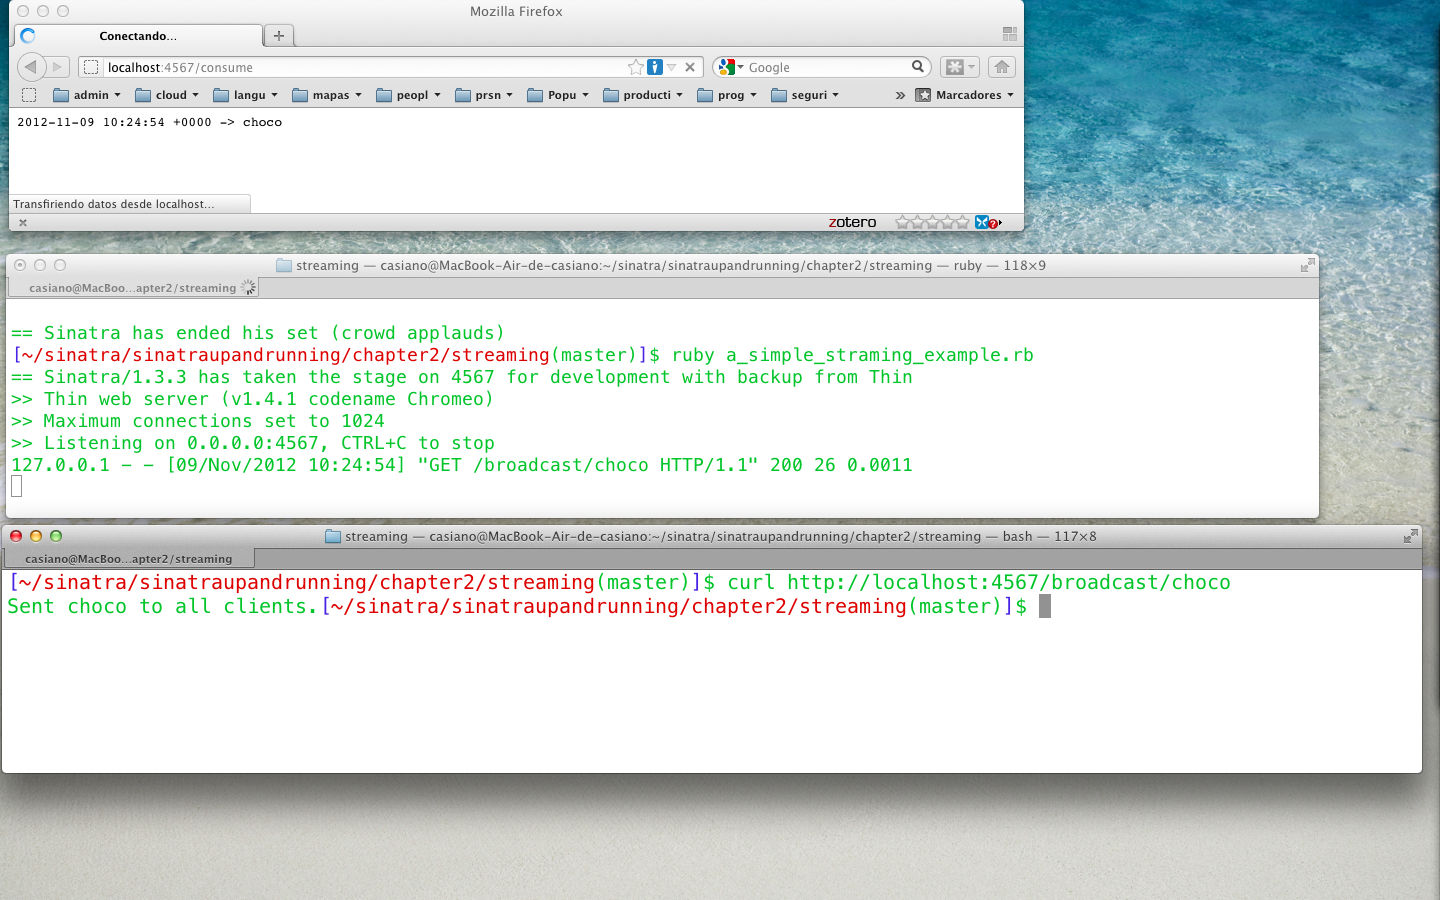
\includegraphics[scale=0.6]{sinatra/chapter2fundamentos/streamingbroadcast.png}
%\end{center}
%\label{figure:broadcaststreaming}
%\caption{Manteniendo una Conexión Abierta}
%\end{figure}

\begin{enumerate}
\item 
Este ejemplo usa
\eventmachine{}.
\item 
\eventmachine {} 
is a library for Ruby, C++, and Java programs. 
\item 
It provides event-driven I/O using the \wikip{Reactor pattern}{Reactor\_pattern}. 
\begin{enumerate}
\item 
The \cei{reactor design pattern} is an event handling pattern for
handling service requests delivered concurrently to a service handler
by one or more inputs.
\item 
The service handler then demultiplexes the incoming requests and
dispatches them synchronously to the associated request handlers.
\end{enumerate}
\item 
El módulo
\htmladdnormallink{Module: EventMachine::Deferrable}{http://eventmachine.rubyforge.org/EventMachine/Deferrable.html}
provee el método \verb|(Object) callback(&block)|.
y el método \verb|(Object) errback(&block)| 
\begin{enumerate}
\item 
El método \verb|(Object) callback(&block)|
specifies a block to be executed if and when the Deferrable object receives a status of \verb|:succeeded|.
\begin{verbatim}
    out.callback do 
      logger.warn "connection closed. out = #{out}"
      settings.connections.delete(out) 
      logger.warn "connections.length = #{settings.connections.length}"
    end
\end{verbatim}
\item 
El método \verb|(Object) errback(&block)| 
specifies a block to be executed if and when the Deferrable object receives
a status of \verb|:failed|.
\begin{verbatim}
    out.errback do
      logger.warn "we just lost  connection!. out = #{out}"
      settings.connections.delete(out)
      logger.warn "connections.length = #{settings.connections.length}"
    end
\end{verbatim}
\item 
\eventmachine{} (EM) adds two different formalisms for lightweight concurrency to the Ruby programmer’s toolbox: spawned processes and \cei{deferrables}.
\end{enumerate}
\end{enumerate}


\section{Streaming y Valores de Retorno}


El valor de retorno del bloque de una ruta determina
el cuerpo de respuesta pasado al cliente HTTP, o al menos al siguiente middleware en la pila de Rack.
Lo habitual es que sea una \verb|String| pero puede ser otra cosa.

De hecho, podemos retornar cualquier tipo de objeto que sea una respuesta Rack válida,
un objeto que disponga de un \verb|each| o un código de estatus HTTP:

\begin{itemize}
\item
Un \verb|Array| con tres elementos: \verb|[status (Fixnum), headers (Hash), response body (responds to #each)]|

\item
Un \verb|Array| con dos elementos:
 \verb|[status (Fixnum), response body (responds to #each)]|

\item
Un objeto que responde a \verb|#each| y que le pasa strings al bloque dado

\item
Un \verb|Fixnum| que representa el status code
\end{itemize}

Así podemos, implementar el siguiente ejemplo que funciona en streaming cuando se usa con 
\verb|puma|:

\begin{verbatim}
[~/sinatra/sinatra-streaming/intro-streaming(master)]$ cat stream.rb 
require 'sinatra'

before do
  content_type :txt
end

class Flujo
  def each
    5.times do |i| 
      yield "#{i}: #{Time.now}\n"
      sleep 1
    end
  end
end

get '/' do
  puts env
  Flujo.new
end
\end{verbatim}
Véase el código en
\htmladdnormallink{https://github.com/crguezl/sinatra\_intro/tree/master/streaming}{https://github.com/crguezl/sinatra\_intro/tree/master/streaming}.

\begin{verbatim}
[~/sinatra/sinatra-streaming/intro-streaming(master)]$ cat Rakefile 
task :default => :puma
desc "run stream.rb using puma server"
task :puma do
  sh "ruby stream.rb -e production -s puma"
end

desc "run stream.rb using thin server"
task :thin do
  sh "ruby stream.rb -e production -s thin"
end
\end{verbatim}

\begin{verbatim}
[~/sinatra/sinatra-streaming/intro-streaming(master)]$ rake
ruby stream.rb -e production -s puma
Puma 2.6.0 starting...
* Min threads: 0, max threads: 16
* Environment: development
* Listening on tcp://0.0.0.0:4567
== Sinatra/1.4.4 has taken the stage on 4567 for production with backup from Puma
127.0.0.1 - - [01/Dec/2013 21:05:32] "GET / HTTP/1.1" 200 - 5.0094
\end{verbatim}
Nota: con \verb|thin| no funciona en modo streaming Prepara la página completa y la suelta
de golpe.

Cuando visitamos \verb|localhost:4567| obtenemos una salida en la que cada línea
aparece un segundo después que la anterior:
\begin{verbatim}
0: 2013-12-01 21:05:27 +0000
1: 2013-12-01 21:05:28 +0000
2: 2013-12-01 21:05:29 +0000
3: 2013-12-01 21:05:30 +0000
4: 2013-12-01 21:05:31 +0000
\end{verbatim}

\section{Sinatra usando Streaming, Rack MiddleWare y map}

Véase el código en 
\htmladdnormallink{sinatra\_intro/streaming/better\_middleware\_handling.rb}{https://github.com/crguezl/sinatra_intro/blob/master/streaming/better_middleware_handling.rb}
en GitHub.

Otro beneficio que obtenemos cuando usamos Sinatra::Streaming (parte de Sinatra::Contrib) es que:

Blocks passed to \verb|#map!| or 
\verb|#map| will actually be applied when streaming takes place (véase 
\htmladdnormallink{http://www.sinatrarb.com/contrib/streaming.html}{http://www.sinatrarb.com/contrib/streaming.html}:

\begin{verbatim}
[~/sinatra/sinatra-streaming/intro-streaming(master)]$ cat better_middleware_handling.rb 
# http://www.sinatrarb.com/contrib/streaming.html

require 'sinatra'
require 'sinatra/streaming'

class StupidMiddleware
  def initialize(app) 
    @app = app 
  end

  def call(env)
    status, headers, body = @app.call(env)
    # Blocks passed to #map! or #map will actually be applied when streaming takes place
    body.map! { |e| e.upcase }
    [status, headers, body]
  end
end

use StupidMiddleware

before do
  content_type :html
end

song = %q{
And now, the end is near 
And so I face the final curtain 
My friend, I'll say it clear 
I'll state my case, of which I'm certain 
I've lived a life that's full 
I traveled each and ev'ry highway 
And more, much more than this, I did it my way 

Regrets, I've had a few 
But then again, too few to mention 
I did what I had to do , I saw it through without exemption 
I planned each charted course, each careful step along the highway 
And more, much more than this, I did it my way 

Yes, there were times, I'm sure you knew 
When I bit off more than I could chew 
And through it all, when there was doubt 
I ate it up and spit it out 
I faced it all and I stood tall and did it my way 

I've loved, I've laughed and cried 
I've had my fill, my share of losing 
And now, as tears subside, I find it all so amusing 
To think I did all that 
And may I say, not in a shy way, 
"Oh, no, oh, no, not me, I did it my way" 

For what is a man, what has he got? 
If not himself, then he has naught 
The right to say the things he feels and not the words of one who kneels 
The record shows I took the blows and did it my way!
}.split(/\n/)

song.map! { |x| x.split(/\s+/) }

set :song, song
set :colors, ["red", "blue", "black", "green", "yellow", "blueviolet" ]

get '/' do
  color = 0
  stream do |out|
    out.puts '<pre>'
    settings.song.each do |line|
      line.each do |w|
        out.print %Q{<font color="#{settings.colors[color]}">#{w} </font>}
        color = (color+1) % settings.colors.size
        sleep 0.02
      end
      out.puts "\n"
      sleep 1
   end
   out.puts '</pre>'
   out.close
  end
end
\end{verbatim}

\section{Enlaces Relacionados}

\begin{itemize}
\item
\htmladdnormallink{Streaming Responses}{http://www.sinatrarb.com/intro.html\#Streaming\%20Responses} at Sinatra Intro
\item
\htmladdnormallink{Sinatra::Streaming}{http://www.sinatrarb.com/contrib/streaming.html}
%\item
%\htmladdnormallink{redis + sinatra + rainbows streaming of server-sent events}{http://youtu.be/vwPdZWklykU} YouTube
\end{itemize}

\section{A simple demonstration of streaming Redis pub/sub data}
Véase:
\begin{enumerate}
\item
\htmladdnormallink{A simple demonstration of streaming Redis pub/sub data over HTTP via Sinatra's streaming capabilities.}{https://github.com/gorsuch/sinatra-streaming-example}
\item
\htmladdnormallink{A simple demonstration of streaming Redis pub/sub data over HTTP via Sinatra's streaming capabilities.}{https://github.com/crguezl/sinatra-streaming-example} forked version crguezl
\item Véa el capítulo {\it Redis y Sinatra} \ref{chapter:redisysinatra}
\item 
\htmladdnormallink{redis}{https://github.com/redis/redis-rb} gem en GitHub
\item 
\htmladdnormallink{redis}{http://rubydoc.info/gems/redis/3.0.6/frames} documentación de la gema
\item 
\htmladdnormallink{Redis Pub/Sub}{http://redis.io/topics/pubsub}
\item 
\htmladdnormallink{Redis::Subscription}{http://rubydoc.info/gems/redis/3.0.6/Redis/Subscription}:
\item 
\htmladdnormallink{Heroku addon Redis To Go}{https://addons.heroku.com/redistogo}
\end{enumerate}

\parrafo{web.rb}
\begin{verbatim}
[~/sinatra/sinatra-streaming/sinatra-streaming-example(master)]$ cat web.rb
require 'redis'
require 'sinatra'

configure do
  redis_url = ENV["REDISTOGO_URL"] || "redis://localhost:6379"
  uri = URI.parse(redis_url)
  set :redis, Redis.new(:host => uri.host, :port => uri.port, :password => uri.password)
end

get '/' do
  "<pre>curl -v https://sinatra-streaming-example.herokuapp.com/stream</pre>"
end

get '/stream' do
  puts "connection made"

  stream do |out|
    settings.redis.subscribe 'time' do |on|
      on.message do |channel, message|
        out << "#{message}\n"
      end
    end
  end
end
\end{verbatim}
\Redis{} is a key-value store; it supports lists, hashes, sets, and ordered sets.

El código 
\begin{verbatim}
  redis_url = ENV["REDISTOGO_URL"] || "redis://localhost:6379"
\end{verbatim}
decide si estamos en Heroku o no. Si estamos en Heroku deberemos haber instalado
el \htmladdnormallink{Heroku addon Redis To Go}{https://addons.heroku.com/redistogo}.


La llamada:
\begin{verbatim}
  set :redis, Redis.new(:host => uri.host, :port => uri.port, :password => uri.password)
\end{verbatim}
conecta con el servidor Redis.

The Redis class exports methods that are named identical to the
commands they execute. The arguments these methods accept are often
identical to the arguments specified on the Redis website.

In Redis,
\verb|SUBSCRIBE|, \verb|UNSUBSCRIBE| and \verb|PUBLISH| implement 
the \wikip{Publish/Subscribe}{Publish/subscribe} messaging paradigm where 
\begin{enumerate}
\item 
In the \cei{Publish/Subscribe} pattern, senders (publishers) are not programmed to send their messages to
specific receivers (subscribers). 
\item 
Rather, published messages are
characterized into channels, without knowledge of what (if any)
subscribers there may be. 
\item 
Subscribers express interest in one or
more channels, and only receive messages that are of interest,
without knowledge of what (if any) publishers there are. 
\item 
This
decoupling of publishers and subscribers can allow for greater
scalability and a more dynamic network topology.
\end{enumerate}
For instance in order to subscribe to channels \verb|foo| and \verb|bar| the
client issues a \verb|SUBSCRIBE| providing the names of the channels:
\begin{verbatim}
SUBSCRIBE foo bar
\end{verbatim}

Messages sent by other clients to these channels will be pushed by
Redis to all the subscribed clients.

A client subscribed to one or more channels should not issue commands,
although it can subscribe and unsubscribe to and from other channels.

The reply of the \verb|SUBSCRIBE| and \verb|UNSUBSCRIBE| operations are sent in
the form of messages, so that the client can just read a coherent
stream of messages where the first element indicates the type of
message.

El objeto \verb|on| pasado al bloque está en la clase
\htmladdnormallink{Redis::Subscription}{http://rubydoc.info/gems/redis/3.0.6/Redis/Subscription}:
\begin{verbatim}
    settings.redis.subscribe 'time' do |on|
      on.message do |channel, message|
        out << "#{message}\n"
      end
\end{verbatim}
el objeto \verb|on| dispone del método \verb|message| que establece una callback
que será ejecutada cada vez que se produzca un mensaje.

\parrafo{worker.rb}
\begin{verbatim}
[~/sinatra/sinatra-streaming/sinatra-streaming-example(master)]$ cat worker.rb 
require 'uri'
require 'redis'

redis_url = ENV["REDISTOGO_URL"] || "redis://localhost:6379"
uri = URI.parse(redis_url)
r = Redis.new(:host => uri.host, :port => uri.port, :password => uri.password)

while true do
  puts "publishing..."
  r.publish "time", Time.now.utc
  sleep 1  
end
\end{verbatim}

\parrafo{Procfile}
\begin{verbatim}
[~/sinatra/sinatra-streaming/sinatra-streaming-example(master)]$ cat Procfile 
web: bundle exec ruby web.rb -p $PORT
worker: bundle exec ruby worker.rb
\end{verbatim}
The \verb|web| process type, describes to Heroku how to start the web application server.

\htmladdnormallink{An interesting thing to mention here is that Heroku}{http://www.neilmiddleton.com/the-procfile-is-your-friend/}
only auto-launches
the web process in your Procfile when deploying, whereas \verb|foreman|
launches everything. 

\parrafo{Gemfile}
\begin{verbatim}
[~/sinatra/sinatra-streaming/sinatra-streaming-example(master)]$ cat Gemfile
source 'https://rubygems.org'

gem 'foreman'
gem 'redis'
gem 'sinatra'
gem 'thin'
\end{verbatim}

\parrafo{Ejecución: Arranca el Servidor Redis}

\begin{verbatim}
[~/sinatra/sinatra-streaming/sinatra-streaming-example(master)]$ redis-server 
[5604] 04 Dec 10:18:58.126 # Warning: no config file specified, using the default config. In order to specify a config file use redis-server /path/to/redis.conf
[5604] 04 Dec 10:18:58.129 * Max number of open files set to 10032
                _._                                                  
           _.-``__ ''-._                                             
      _.-``    `.  `_.  ''-._           Redis 2.6.14 (00000000/0) 64 bit
  .-`` .-```.  ```\/    _.,_ ''-._                                   
 (    '      ,       .-`  | `,    )     Running in stand alone mode
 |`-._`-...-` __...-.``-._|'` _.-'|     Port: 6379
 |    `-._   `._    /     _.-'    |     PID: 5604
  `-._    `-._  `-./  _.-'    _.-'                                   
 |`-._`-._    `-.__.-'    _.-'_.-'|                                  
 |    `-._`-._        _.-'_.-'    |           http://redis.io        
  `-._    `-._`-.__.-'_.-'    _.-'                                   
 |`-._`-._    `-.__.-'    _.-'_.-'|                                  
 |    `-._`-._        _.-'_.-'    |                                  
  `-._    `-._`-.__.-'_.-'    _.-'                                   
      `-._    `-.__.-'    _.-'                                       
          `-._        _.-'                                           
              `-.__.-'                                               

[5604] 04 Dec 10:18:58.129 # Server started, Redis version 2.6.14
[5604] 04 Dec 10:18:58.129 * The server is now ready to accept connections on port 6379
\end{verbatim}

\parrafo{Ejecución 2: Arranca la aplicación Sinatra y el Worker}
Obsérvese como \verb|bundle exec foreman start| arranca tanto a \verb|worker| como 
a \verb|web|:

\begin{verbatim}
[~/sinatra/sinatra-streaming/sinatra-streaming-example(master)]$ bundle exec foreman start
10:19:04 web.1     | started with pid 5606
10:19:04 worker.1  | started with pid 5607
10:19:05 worker.1  | publishing...
10:19:06 web.1     | == Sinatra/1.3.0 has taken the stage on 5000 for development with backup from Thin
10:19:06 web.1     | >> Thin web server (v1.2.11 codename Bat-Shit Crazy)
10:19:06 web.1     | >> Maximum connections set to 1024
10:19:06 web.1     | >> Listening on 0.0.0.0:5000, CTRL+C to stop
10:19:06 worker.1  | publishing...
10:19:07 worker.1  | publishing...
10:19:08 worker.1  | publishing...
..................................
10:19:37 worker.1  | publishing...
10:19:38 web.1     | connection made
10:19:39 worker.1  | publishing...
..................................
\end{verbatim}

\parrafo{Ejecución 3: Arranca un Cliente}
\begin{verbatim}
[~/sinatra/sinatra-streaming/sinatra-streaming-example(master)]$ curl -v http://localhost:5000/stream
* Adding handle: conn: 0x7fc71280aa00
* Adding handle: send: 0
* Adding handle: recv: 0
* Curl_addHandleToPipeline: length: 1
* - Conn 0 (0x7fc71280aa00) send_pipe: 1, recv_pipe: 0
* About to connect() to localhost port 5000 (#0)
*   Trying 127.0.0.1...
* Connected to localhost (127.0.0.1) port 5000 (#0)
> GET /stream HTTP/1.1
> User-Agent: curl/7.30.0
> Host: localhost:5000
> Accept: */*
> 
< HTTP/1.1 200 OK
< X-Frame-Options: sameorigin
< X-XSS-Protection: 1; mode=block
< Content-Type: text/html;charset=utf-8
< Connection: close
* Server thin 1.2.11 codename Bat-Shit Crazy is not blacklisted
< Server: thin 1.2.11 codename Bat-Shit Crazy
< 
2013-12-04 13:24:13 UTC
2013-12-04 13:24:14 UTC
2013-12-04 13:24:15 UTC
2013-12-04 13:24:16 UTC
2013-12-04 13:24:17 UTC
.......................
\end{verbatim}

\section{Comet}

\cei{Comet} is a web application architecture in which a long-held HTTP
request allows a web server to push data to a browser, without the
browser explicitly requesting it.

In Ajax the client pulls data from the server. With Comet the server pushes data to the client.

Other names for Comet are
\begin{enumerate}
\item 
\cei{Server Push}
\item 
\cei{Ajax Push}
\item 
\cei{HTTP Streaming}
\end{enumerate}

\cei{Server Sent Events} defines a simple Comet API in the form of a \EventSource{}
object.
Server-Sent Events (SSE) is a standard describing how servers can initiate data transmission towards clients once an initial client connection has been established. 

The Server-Sent Events draft standard defines an \EventSource{} that makes Comet applications
easy to write.

\begin{verbatim}
var ticker = new EventSource("stockprices.php"); 
ticker.onmessage = function(e) {
  var type = e.type; 
  var data = e.data;
  // Now process the event type and event data strings. 
}
\end{verbatim}

The event object associated with a message event has a \verb|data| property
that holds whatever the server sent as the payload for this event.

The \verb|type| property by default is \verb|"message"| but the event source 
can sepcify a different string for the property.

A single \verb|onmessage| event handler receives all events from a given server event
source, and can dispatch them, if necessary, based on their \verb|type| property.

\section{Chat Utilizando Streaming y Server Sent Events (SSE)}
\label{section:chatutilizandostreaming}


Los fuentes de este ejemplo se encuentran en la rama \verb|original| del repositorio
\htmladdnormallink{sinatra-streaming-example-chat}{https://github.com/crguezl/sinatra-streaming-example-chat/tree/original}.
La rama \verb|simple| en
\htmladdnormallink{https://github.com/crguezl/sinatra-streaming-example-chat/tree/simple}{https://github.com/crguezl/sinatra-streaming-example-chat/tree/simple}
contiene una versión equivalente pero con los templates separados.

\begin{verbatim}
[~/srcSTW/streaming/chat_with_streaming(master)]$ cat -n chat.rb 
 1  # coding: utf-8
 2  require 'sinatra'
 3  set server: 'thin', connections: []
 4  
 5  get '/' do
 6    halt erb(:login) unless params[:user]
 7    erb :chat, locals: { user: params[:user].gsub(/\W/, '') }
 8  end
\end{verbatim}
Cuando se visita la raíz la primera vez \verb|params[:user]| es \verb|nil|
y se muestra el formulario definido en \verb|login.erb| que obtiene un alias
para el usuario:
\begin{verbatim}
[~/sinatra/sinatra-streaming/chat_with_streaming(simple)]$ cat views/login.erb 
<form action='/' method='GET'>
  <label for='user'>User Name:</label>
  <input name='user' value='' autofocus/>
  <input type='submit' value="GO!" />
</form>
\end{verbatim}
El atributo \verb|for='user'| de \verb|label| indica que esta etiqueta está asociada
con el campo \verb|input| cuyo atributo \verb|name| es \verb|user|.

Una vez que el \verb|<input name='user'>| es rellenado el formulario es procesado por la misma
ruta \verb|/| que ahora muestra el resultado de la plantilla \verb|chat|. 
\begin{verbatim}
10  get '/stream', provides: 'text/event-stream' do
11    stream :keep_open do |out|
12      settings.connections << out
13      out.callback { settings.connections.delete(out) }
14    end
15  end
\end{verbatim}
Routes may include a variety of matching conditions, such as the user \verb|agent:|,
\verb|:host_name| and \verb|:provides|:
\begin{verbatim}
get '/', :provides => ['rss', 'atom', 'xml'] do
  builder :feed
end
\end{verbatim}
Sending an event stream from the source is a matter of constructing
a plaintext response, served with a \verb|text/event-stream| Content-Type,
that follows the Server Sent Event (SSE) format. 

Sigamos:
\begin{verbatim}
16  
17  post '/' do
18    settings.connections.each { |out| out << "data: #{params[:msg]}\n\n" }
19    204 # response without entity body
20  end
\end{verbatim}

\noindent {\bf 204 No Content}

The server has fulfilled the request but does not need to return
an entity-body, and might want to return updated metainformation.

If the client is a user agent, it SHOULD NOT change its document
view from that which caused the request to be sent. This response
is primarily intended to allow input for actions to take place
without causing a change to the user agent's active document view,
although any new or updated metainformation SHOULD be applied to
the document currently in the user agent's active view.

The 204 response MUST NOT include a message-body, and thus is always
terminated by the first empty line after the header fields.
\begin{verbatim}
21  
22  __END__
23  
24  @@ layout
25  <html>
26    <head> 
27      <title>Super Simple Chat with Sinatra</title> 
28      <meta charset="utf-8" />
29      <script src="http://ajax.googleapis.com/ajax/libs/jquery/1/jquery.min.js"></script> 
30    </head> 
31    <body><%= yield %></body>
32  </html>
\end{verbatim}

The \verb|<script>| tag is used to define a client-side script, such as a JavaScript.

The \verb|<script>| element either contains scripting statements, or it points to an external script file through the \verb|src| attribute.

Common uses for JavaScript are image manipulation, form validation, and dynamic changes of content.

The \htmladdnormallink{Google Hosted Libraries}{https://developers.google.com/speed/libraries/devguide} is a content distribution network for
the most popular, open-source JavaScript libraries. To add a library
to your site, simply use \verb|<script>| tags to include the library.
See \htmladdnormallink{https://developers.google.com/speed/libraries/devguide}{https://developers.google.com/speed/libraries/devguide\#jquery}:
\begin{verbatim}
jQuery
snippet: <script src="//ajax.googleapis.com/ajax/libs/jquery/1.8.3/jquery.min.js"></script>
site: http://jquery.com/
versions: 1.8.3, 1.8.2, 1.8.1, 1.8.0, ...
note: 1.2.5 and 1.2.4 are not hosted due to their short and unstable lives in the wild.
\end{verbatim}

\htmladdnormallink{jQuery}{http://docs.jquery.com/} is a fast and concise JavaScript Library that simplifies
HTML document traversing, event handling, animating, and Ajax
interactions for rapid web development.

\verb|jquery.min.js| is a minified version of the \htmladdnormallink{JQuery JavaScript library}{http://docs.jquery.com/},
which provides a number of basic functions for websites. 


\begin{verbatim}
34  @@ login
35  <form action='/'>
36    <label for='user'>User Name:</label>
37    <input name='user' value='' />
38    <input type='submit' value="GO!" />
39  </form>
40  
41  @@ chat
42  <pre id='chat'></pre>
43  
44  <script>
45    // reading
46    var es = new EventSource('/stream');
47    es.onmessage = function(e) { $('#chat').append(e.data + "\n") };
48  
49    // writing
50    $("form").live("submit", function(e) {
51      $.post('/', {msg: "<%= user %>: " + $('#msg').val()});
52      $('#msg').val(''); $('#msg').focus();
53      e.preventDefault();
54    });
55  </script>
56  
57  <form>
58    <input id='msg' placeholder='type message here...' />
59  </form>
\end{verbatim}
\begin{itemize}
\item
\cei{Server-Sent Events (SSE)} are a standard describing how servers can
initiate data transmission towards clients once an initial client
connection has been established. 
\item
They are commonly used to send
message updates or continuous data streams to a browser client and
designed to enhance native, cross-browser streaming through a
JavaScript API called \htmladdnormallink{EventSource}{https://developer.mozilla.org/en/Server-sent_events/EventSource}, 
through which a client requests
a particular URL in order to receive an event stream.
\item
The idea behind \cei{SSE}s is natural: a web app "subscribes" to a
stream of updates generated by a server and, whenever a new event
occurs, a notification is sent to the client. 
\item
When communicating using SSEs, a server can push data to your app
whenever it wants, without the need to make an initial request. In
other words, updates can be streamed from server to client as they
happen. 
\item
SSEs open a \emph{single unidirectional channel} between server
and client.
\item
A Ruby/EventMachine based server implementation for WebSocket and Server-Sent Events is
provided by \htmladdnormallink{Cramp}{http://cramp.in/documentation}.
\item
The \cei{EventSource} interface is used to manage \cei{server-sent events}. 
The server-sent event API is contained in the
\htmladdnormallink{EventSource}{https://developer.mozilla.org/en/Server-sent_events/EventSource}
interface.
\end{itemize}

\begin{itemize}
\item
To open a connection to the server to begin receiving events from
it, you create a new \verb|EventSource| object, specifying the URI of a
script that generates the events:
\begin{verbatim}
      var es = new EventSource('/stream')
\end{verbatim}


\item
Next, we set up a handler for the message event.

When updates are pushed from the server, the \verb|onmessage| handler fires
and new data is available in its \verb|e.data| property:

\begin{verbatim}
47    es.onmessage = function(e) { $('#chat').append(e.data + "\n") };
\end{verbatim}
\item
The magical
part is that whenever the connection is closed, the browser will
automatically reconnect to the source after \verb|~3| seconds. Your server
implementation can even have control over this reconnection timeout.

\item
You can
also call \verb|addEventListener()| to listen for events just like any
other event source:

\begin{verbatim}
source.addEventListener('message', function(e) {
  console.log(e.data);
}, false);

source.addEventListener('open', function(e) {
  // Connection was opened.
}, false);

source.addEventListener('error', function(e) {
  if (e.readyState == EventSource.CLOSED) {
    // Connection was closed.
  }
}, false);
\end{verbatim}

\item
Código HTML generado:
\begin{verbatim}
<html>
  <head> 
    <title>Super Simple Chat with Sinatra</title> 
    <meta charset="utf-8" />
    <script src="http://ajax.googleapis.com/ajax/libs/jquery/1/jquery.min.js"></script> 
  </head> 
  <body><pre id='chat'></pre>

<script>
  // reading
  var es = new EventSource('/stream');
  es.onmessage = function(e) { $('#chat').append(e.data + "\n") };

  // writing
  $("form").live("submit", function(e) {
    $.post('/', {msg: "casiano: " + $('#msg').val()});
    $('#msg').val(''); $('#msg').focus();
    e.preventDefault();
  });
</script>

<form>
  <input id='msg' placeholder='type message here...' />
</form></body>
</html>
\end{verbatim}
\end{itemize}

\begin{itemize}
\item
We start with the dollar sign and parentheses:
\verb|$("form")| to specify a selector. 
The dollar sign ( \verb|$| ) is simply shorthand for jQuery.
With \verb|$("form")| we select all the elements with tag name \verb|form|

\item
\begin{verbatim}
.append( content [, content] )
\end{verbatim}
  \begin{itemize}
  \item
  \verb|content|: \wikip{DOM}{Document\_Object\_Model} element, HTML string, or jQuery object to insert
  at the end of each element in the set of matched elements.

  \item
  \verb|content|: One or more additional \cei{DOM} elements, arrays of
  elements, HTML strings, or jQuery objects to insert at the end of
  each element in the set of matched elements.
  \end{itemize}

\item
\begin{verbatim}
.live( events, handler(eventObject) ) Returns: jQuery
\end{verbatim}
Description: Attach an event handler for all elements which match the current selector, now and in the future.

  \begin{itemize}
  \item
  \verb|events|: A string containing a \htmladdnormallink{JavaScript event type}{http://www.w3schools.com/js/js_htmldom_events.asp}, such as \verb"click" or \verb"keydown." 
  As of jQuery 1.4 the string can contain multiple, space-separated event types or custom event names.
  \item
  \verb|handler(eventObject)|: A function to execute at the time the event is triggered.

    \item 
    As of jQuery 1.7, the \verb|.live()| method is deprecated. 
    Use \verb|.on()| to attach event handlers. 

    These are equivalent templates:

    \begin{verbatim}
    $( selector ).live( events, data, handler );                // jQuery 1.3+
    $( document ).on( events, selector, data, handler );        // jQuery 1.7+
    \end{verbatim}
    The \verb|events| argument can either be a space-separated list of event
    type names and optional namespaces, or an object of event name
    strings and handlers. The \verb|data| argument is optional and can be
    omitted.
  \end{itemize}
\item
\begin{verbatim}
jQuery.post( url [, data] [, success(data, textStatus, jqXHR)] [, dataType] )
\end{verbatim}
  \begin{itemize}
  \item
  \verb|url|: A string containing the URL to which the request is sent.
  \item
  \verb|data|: A map or string that is sent to the server with the request.
  \item
  \verb|success(data, textStatus, jqXHR)|: A callback function that is executed if the request succeeds.
  \item
  \verb|dataType|: The type of data expected from the server. Default: Intelligent Guess (xml, json, script, text, html).
  \end{itemize}

This is an easy way to send a simple \verb|POST| request to a server.
It allows a single callback function to be specified that will be executed when the
request is complete (and only if the response has a successful
response code).

\verb|$.post()| returns the \verb|XMLHttpRequest| that it creates. In most cases
you won't need that object to manipulate directly, but it is available
if you need to abort the request manually.

\item
\begin{verbatim}
.val
\end{verbatim}

Get the input value of the first matched element.

A value is returned for all input elements, including selects and textareas. 
For multiple selects an array of values is returned.

For example:

\begin{verbatim}
$('select.foo option:selected').val();    // get the value from a dropdown select
$('select.foo').val();                    // get the value from a dropdown select even easier
$('input:checkbox:checked').val();        // get the value from a checked checkbox
$('input:radio[name=bar]:checked').val(); // get the value from a set of radio buttons
\end{verbatim}


\item
\begin{verbatim}
.focus( handler(eventObject) )
.focus( [eventData], handler(eventObject) )
.focus()
\end{verbatim}
\verb|handler(eventObject)|: A function to execute each time the event is triggered.
\verb|eventData|: A map of data that will be passed to the event handler.

This method is a shortcut for \verb|.trigger('focus')|.
The focus event is sent to an element when it gains focus. 
This event is implicitly applicable to a limited set of elements, such as form elements 
(\verb|<input>|, \verb|<select>|, etc.) and links (\verb|<a href>|). In recent browser
versions, the event can be extended to include all element types
by explicitly setting the element's tabindex property. An element
can gain focus via keyboard commands, such as the Tab key, or by
mouse clicks on the element.
Elements with focus are usually highlighted in some way by the
browser, for example with a dotted line surrounding the element.
The focus is used to determine which element is the first to receive
keyboard-related events.

\item
\begin{verbatim}
event.preventDefault() Returns: undefined
\end{verbatim}
Description: If this method is called, the default action of the
event will not be triggered.

For example, clicked anchors will not take the browser to a new
URL. We can use \verb|event.isDefaultPrevented()| to determine if this
method has been called by an event handler that was triggered by
this event.
\end{itemize}



\begin{figure}[htb]
\begin{center}
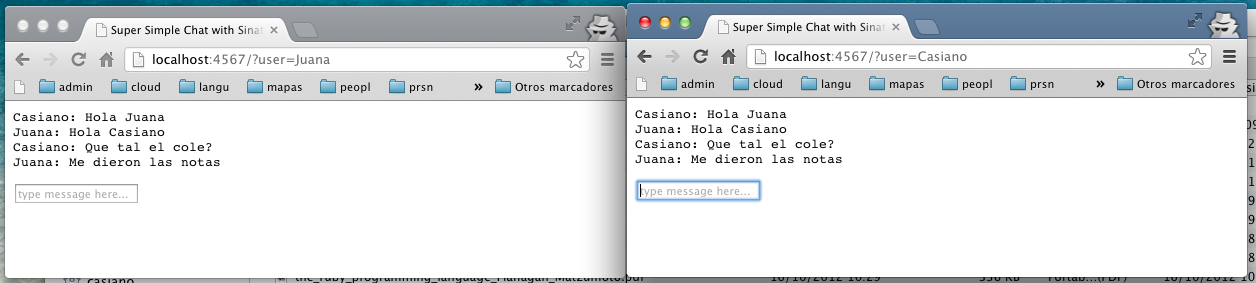
\includegraphics[scale=0.7]{sinatra/chapter2fundamentos/sinatra_chat.png}
\end{center}
\label{figure:sinatrachat}
\caption{Chat en Sinatra Usando Streaming}
\end{figure}

\subsection{Enlaces Relacionados}

\begin{itemize}
\item 
\htmladdnormallink{Real Time Rack por Konstantin Haase}{http://confreaks.com/videos/727-rockymtnruby2011-real-time-rack} en 
\htmladdnormallink{http://confreaks.com/}{http://confreaks.com/}
\item 
\htmladdnormallink{Slides for "Real Time Rack"}{https://github.com/rkh/presentations/tree/realtime-rack}. Contains the example used in the presentations.
It is also of how to use Scott Chacon 
\htmladdnormallink{showoff}{https://github.com/schacon/showoff}
presentation software
\item 
El blog de 
\htmladdnormallink{Konstantin Haase}{http://rkh.im/} desarrollador al cargo de Sinatra
\item 
\htmladdnormallink{Konstantin Haase en GitHub}{https://github.com/rkh?tab=repositories}
\item
\htmladdnormallink{Simple Chat Application using the Sinatra Streaming API}{https://gist.github.com/1476463}
\item
\htmladdnormallink{Stream Updates With Server-Sent Events}{http://www.html5rocks.com/en/tutorials/eventsource/basics/}
\item
\htmladdnormallink{Using server-sent events}{https://developer.mozilla.org/en-US/docs/Server-sent_events/Using_server-sent_events}
\item
\htmladdnormallink{EventSource}{https://developer.mozilla.org/en-US/docs/Server-sent_events/EventSource}
\item
\htmladdnormallink{Chat Server with server-sent Events}{http://aaltowebapps.com/websocketsChatSSE.html}
\item
\htmladdnormallink{A shared canvas where multiple clients can draw lines using}{http://aaltowebapps.com/websocketsDrawEM.html}
\htmladdnormallink{EM-Websocket}{https://github.com/igrigorik/em-websocket}
\item
\htmladdnormallink{JQuery documentation}{http://docs.jquery.com/}
\item
\htmladdnormallink{What is the Document Object Model?}{http://www.w3.org/TR/DOM-Level-2-Core/introduction.html}
\item
\htmladdnormallink{JavaScript and HTML DOM Reference}{http://www.w3schools.com/jsref/default.asp}
\end{itemize}

\subsection{Código Completo del Chat}
\begin{verbatim}
[17:51][~/srcSTW/streaming/chat_with_streaming(master)]$ cat chat.rb 
# coding: utf-8
require 'sinatra'
set server: 'thin', connections: []

get '/' do
  halt erb(:login) unless params[:user]
  erb :chat, locals: { user: params[:user].gsub(/\W/, '') }
end

get '/stream', provides: 'text/event-stream' do
  stream :keep_open do |out|
    settings.connections << out
    out.callback { settings.connections.delete(out) }
  end
end

post '/' do
  settings.connections.each { |out| out << "data: #{params[:msg]}\n\n" }
  204 # response without entity body
end

__END__

@@ layout
<html>
  <head> 
    <title>Super Simple Chat with Sinatra</title> 
    <meta charset="utf-8" />
    <script src="http://ajax.googleapis.com/ajax/libs/jquery/1/jquery.min.js"></script> 
  </head> 
  <body><%= yield %></body>
</html>

@@ login
<form action='/'>
  <label for='user'>User Name:</label>
  <input name='user' value='' />
  <input type='submit' value="GO!" />
</form>

@@ chat
<pre id='chat'></pre>

<script>
  // reading
  var es = new EventSource('/stream');
  es.onmessage = function(e) { $('#chat').append(e.data + "\n") };

  // writing
  $("form").live("submit", function(e) {
    $.post('/', {msg: "<%= user %>: " + $('#msg').val()});
    $('#msg').val(''); $('#msg').focus();
    e.preventDefault();
  });
</script>

<form>
  <input id='msg' placeholder='type message here...' />
</form>[
\end{verbatim}

\section{Chat Simple}

\parrafo{Donde}
\begin{itemize}
\item
\begin{verbatim}
[~/sinatra-streaming/blazeeboychat(master)]$ pwd -P
/Users/casiano/local/src/ruby/sinatra/sinatra-streaming/blazeeboychat
[~/sinatra-streaming/blazeeboychat(master)]$ git remote -v
origin  git@github.com:crguezl/chat-blazee.git (fetch)
origin  git@github.com:crguezl/chat-blazee.git (push)
\end{verbatim}
\item
\htmladdnormallink{https://github.com/crguezl/chat-blazee}{https://github.com/crguezl/chat-blazee}
\item
\htmladdnormallink{https://gist.github.com/blazeeboy/9289678}{https://gist.github.com/blazeeboy/9289678}
\end{itemize}

\parrafo{Código}
\begin{verbatim}
[~/sinatra-streaming/blazeeboychat(master)]$ cat chat.rb 
require 'sinatra' # gem install sinatra --no-rdoc --no-ri
set :port, 3000
set :environment, :production
 
html = <<-EOT
<html><head><style>
#text{width:100%; font-size: 15px; padding: 5px; display: block;}
</style></head><body>
  <input id="text" placeholder="Write then press Enter."/>
  <div id="chat"></div>
  <script src="http://code.jquery.com/jquery-1.11.0.min.js"></script>
  <script>
  $('#text').keypress(function(e){
    if( e.keyCode==13 ){
      $.get('/send',{text:$('#text').val()});
      $('#text').val('');
    }
  });
  last = 0;
  setInterval(function(){
    $.get('/update',{last:last},
      function(response){
        last = $('<p>').html(response).find('span').data('last');
        $('#chat').append(response);
        });
    },1000);
  </script>
</body></html>
EOT
 
chat = ['welcome..']
get('/') { html }
get '/send' do
  chat << "#{request.ip} : #{params['text']}"
  nil
end
get '/update' do
  updates = chat[params['last'].to_i..-1]
  last = "<span data-last=\"#{chat.size}\"></span>"
  if updates.size>0
  updates.join('</br>') + "#{last}</br>"
  else
    last
  end
end
\end{verbatim}

\sectionpractica{Chat con Mensajes Individuales}
\label{practica:chat_con_mensajes_uno_uno}
Mejore el chat utilizando streaming y \cei{server sent events} descrito en la sección
\ref{section:chatutilizandostreaming} para que:
\begin{itemize}
\item
Si el usuario escribe en su caja \verb|/nickname: mensaje| ese \verb|mensaje| sólo se entregue 
al usuario \verb|nickname|
\end{itemize}

\sectionpractica{Chat con Estilo}
\label{practica:chat_con_frames}
Mejore la vista del chat utilizando streaming y server sent events descrito en la sección
\ref{section:chatutilizandostreaming} para que:
\begin{itemize}
\item
Usando contenedores
tablas u otros mecanismos, haga que en un marco salgan los nicks de los usuarios conectados,
en otro la conversación y en un tercero el texto que se va a enviar.

\begin{figure}[htb]
\begin{center}
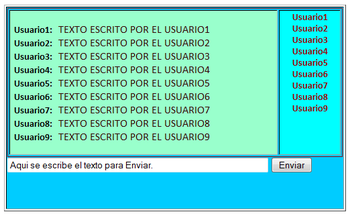
\includegraphics[scale=1]{sinatra/chapter2fundamentos/Chat_web.png}
\end{center}
\label{figure:sinatrachat}
\caption{Típica disposición de un chat}
\end{figure}
\end{itemize}

Mejore la práctica para que puedan producirse conversaciones por pares.

Véase la rama \verb|master| en
\htmladdnormallink{https://github.com/crguezl/sinatra-streaming-example-chat/}{https://github.com/crguezl/sinatra-streaming-example-chat}

\sectionpractica{Chat con TicTacToe}
Modifique la práctica anterior añadiendo un nuevo contenedor en la vista 
con el tablero del tictactoe.

\begin{enumerate}
\item 
Los usuarios tiene dos estados \verb|jugando| (en rojo)
o libres (en \verb|verde|).

\item 
Al cliquear en un usuario libre elegimos jugar con él. 
Se le mostrará a este la opción de aceptar o rechazar
la oferta. 

\item 
Si acepta se comenzará con el juego a dos del tictactoe
actualizando el estado de estos usuarios.

\item 
Al finalizar la partida los jugadores pasan al estado de libres
\end{enumerate}

\section{Embedding Sinatra within EventMachine}

Véase 
\htmladdnormallink{Sinatra Recipes. Embedding Sinatra within EventMachine}{http://recipes.sinatrarb.com/p/embed/event-machine}.

\eventmachine{} is a very useful tool and sometimes you need to add a
web-interface on top of it. Yes, EM does support this out of the
box, but it can be ugly and hard to work with. Why not use something
that everyone already knows and loves like Sinatra?

Below is a (working) code-sample for running a simple HelloWorld
Sinatra app within \EventMachine{}. I've also provided a simple example
of deferring tasks within your Sinatra call.

\begin{verbatim}
[~/sinatra/sinatra-eventmachine]$ cat em-sinatra-test.rb 
require 'eventmachine'
require 'sinatra/base'
require 'thin'


# This example shows you how to embed Sinatra into your EventMachine
# application. This is very useful if you're application needs some
# sort of API interface and you don't want to use EM's provided
# web-server.

def run(opts)

  # Start he reactor
  EM.run do

    # define some defaults for our app
    server  = opts[:server] || 'thin'
    host    = opts[:host]   || '0.0.0.0'
    port    = opts[:port]   || '8181'
    web_app = opts[:app]

    # create a base-mapping that our application will set at. If I
    # have the following routes:
    dispatch = Rack::Builder.app do
      map '/' do
        run web_app
      end
    end

    # NOTE that we have to use an EM-compatible web-server. There
    # might be more, but these are some that are currently available.
    unless ['thin', 'hatetepe', 'goliath'].include? server
      raise "Need an EM webserver, but #{server} isn't"
    end

    # Start the web server. Note that you are free to run other tasks
    # within your EM instance.
    Rack::Server.start({
      app:    dispatch,
      server: server,
      Host:   host,
      Port:   port
    })
  end
end

# Our simple hello-world app
class HelloApp < Sinatra::Base
  # threaded - False: Will take requests on the reactor thread
  #            True:  Will queue request for background thread
  configure do
    set :threaded, false
  end

  # Request runs on the reactor thread (with threaded set to false)
  get '/hello' do
    'Hello World'
  end

  # Request runs on the reactor thread (with threaded set to false)
  # and returns immediately. The deferred task does not delay the
  # response from the web-service.
  get '/delayed-hello' do
    EM.defer do
      sleep 5
    end
    'I\'m doing work in the background, but I am still free to take requests'
  end
end

# start the application
run app: HelloApp.new
\end{verbatim}

You can run this simply with the command:

\begin{verbatim}
ruby em-sinatra-test.rb   # em-sinatra-test.rb is the filename of the above-code
\end{verbatim}
You should also be able to test that it is working correctly with the following \verb|ab| 
command:

\begin{verbatim}
ab -c 10 -n 100 http://localhost:8181/delayed-hello
\end{verbatim}
\cei{ApacheBench} (\tei{ab}) is a single-threaded command line
computer program for measuring the performance of HTTP web servers.
Originally designed to test the Apache HTTP Server, it is generic
enough to test any web server (Véase 
\htmladdnormallink{http://httpd.apache.org/docs/2.2/programs/ab.html}{http://httpd.apache.org/docs/2.2/programs/ab.html}).

If this finishes in \verb|zero point something| seconds, then you have
successfully setup Sinatra to run within EM and you are taking
requests on the event-loop and deferring tasks to the background.

If it takes any longer than that, then you are most likely taking
requests in the background which means when the EM queue fills up,
you can't process your sinatra requests (not a good thing!). Make
sure that you have threaded set to false and then try again.

Here is an execution:
\begin{verbatim}
[~/sinatra/sinatra-eventmachine]$ ab -c 10 -n 100 http://localhost:8181/delayed-hello
This is ApacheBench, Version 2.3 <$Revision: 655654 $>
Copyright 1996 Adam Twiss, Zeus Technology Ltd, http://www.zeustech.net/
Licensed to The Apache Software Foundation, http://www.apache.org/

Benchmarking localhost (be patient).....done


Server Software:        thin
Server Hostname:        localhost
Server Port:            8181

Document Path:          /delayed-hello
Document Length:        70 bytes

Concurrency Level:      10
Time taken for tests:   0.096 seconds
Complete requests:      100
Failed requests:        0
Write errors:           0
Total transferred:      30300 bytes
HTML transferred:       7000 bytes
Requests per second:    1043.96 [#/sec] (mean)
Time per request:       9.579 [ms] (mean)
Time per request:       0.958 [ms] (mean, across all concurrent requests)
Transfer rate:          308.91 [Kbytes/sec] received

Connection Times (ms)
              min  mean[+/-sd] median   max
Connect:        0    0   0.1      0       1
Processing:     2    9  11.6      5      44
Waiting:        1    8  11.7      5      43
Total:          2    9  11.6      6      44

Percentage of the requests served within a certain time (ms)
  50%      6
  66%      6
  75%      7
  80%      7
  90%     44
  95%     44
  98%     44
  99%     44
 100%     44 (longest request)
\end{verbatim}

\parrafo{Véase}
\begin{enumerate}
\item 
\htmladdnormallink{Asynchronous responses in Rack}{http://polycrystal.org/2012/04/15/asynchronous_responses_in_rack.html} por 
\htmladdnormallink{Patrick}{http://polycrystal.org/authors/pat/}
\end{enumerate}

\section{Ejemplo de Server Sent Events: irb en el navegador}

Véase 
\begin{enumerate}
\item 
\htmladdnormallink{Real Time Rack presentation by Konstantin Haase}{https://github.com/rkh/presentations/tree/realtime-rack}
en GitHub using 
Scott Chacon \htmladdnormallink{showoff}{https://github.com/schacon/showoff}
\item 
\htmladdnormallink{The corresponding talk "Real Time Rack" by
Konstantin Haase}{http://confreaks.com/videos/727-rockymtnruby2011-real-time-rack}
2011. Confreaks videos.
%\item \htmladdnormallink{iPad app to present ShowOff presentations from}{https://github.com/schacon/ShowOffPad} % ObjectiveC
\item La sección {\it Showoff} \ref{chapter:showoff} en estos apuntes
\end{enumerate}

Este código se encuentra en:
\htmladdnormallink{https://github.com/rkh/presentations/blob/realtime-rack/example.rb}{https://github.com/rkh/presentations/blob/realtime-rack/example.rb}

El javascript y el server se activan desde las trasparencias. En concreto en esta trasparencia 
que está en el fichero
\verb|slides/01_slides.md|:

\begin{verbatim}
!SLIDE center

# Demo! #

<iframe src="/events?" width="980" height="600"></iframe>

.notes Next: Rack
\end{verbatim}
The \verb|<iframe>| tag specifies an inline frame.
An inline frame is used to embed another document within the current HTML document.

\verb|src="/events?"| hace que se dispare el código correspondiente a la ruta
\verb|/events| descrita en el fichero \verb|example.rb|.

La ruta \verb|/events|
está en el fichero \verb|example.rb|:
\begin{verbatim}
  get('/events') { slim :html }
\end{verbatim}

El fichero \verb|example.rb| es cargado desde el \verb|config.ru|:
\begin{verbatim}
[~/local/src/ruby/sinatra/sinatra-streaming/konstantin_haase/presentations(realtime-rack)]$ cat config.ru 
require 'showoff'
require './example'

use Example
run ShowOff
\end{verbatim}
Obsérvese que es cargado por \verb|config.ru| mediante \verb|use|.

El template \verb|html| contiene:
\begin{verbatim}
@@ html
html
  head
    title brirb
    link href="/events.css" rel="stylesheet" type="text/css"
    script src="/jquery.min.js" type="text/javascript"
    script src="/events.js" type="text/javascript"
  body
    #log
    form#form
      | &gt;&gt;&nbsp;
      input#input type='text'

\end{verbatim}
Como vemos tenemos identificadores \verb|log|, \verb|form| y \verb|input| para hablar
de los correspondientes elementos implicados.

La carga de \verb|/events.js| es también manejado por una ruta:

\begin{verbatim}
   get('/events.js') { coffee :script }
\end{verbatim}
La gema 
\htmladdnormallink{coffee-script}{https://github.com/josh/ruby-coffee-script}
provee el mecanismo para compilar el javascript y producir el correspondiente
código JavaScript.

Este es el CoffeeScript contenido en 
el template \verb|script|:
\begin{verbatim}
$(document).ready ->
  input   = $("#input")
  log     = $("#log")
  history = []
  count   = 0
  output  = (str) ->
    log.append str
    log.append "<br>"
    input.attr scrollTop: input.attr("scrollHeight")

  input.bind "keydown", (e) ->
    if e.keyCode == 38 or e.keyCode == 40
      count += e.keyCode - 39
      count = 0 if count < 0
      count = input.length + 1 if count > input.length
      input.val history[count]
      false
    else
      true

  $("#form").live "submit", (e) ->
    value = input.val()
    history.push value
    count++
    $.post '/run', code: input.val()
    output "&gt;&gt; #{value}"
    input.val ""
    input.focus()
    e.preventDefault()

  src = new EventSource('/events.es')
  src.onmessage = (e) -> output e.data
\end{verbatim}
\begin{enumerate}
\item 
La llamada \verb|output(str)| añade en el punto indicado por 
\verb|#log| el texto \verb|str|. Además se encarga del scrolling:
\begin{verbatim}
  output  = (str) ->
    log.append str
    log.append "<br>"
    input.attr scrollTop: input.attr("scrollHeight")
\end{verbatim}
\item  El método JQuery
\verb|.bind( eventType [, eventData ], handler(eventObject) )|
Attaches a handler to an event for the elements.
En este caso \verb|eventType| es \verb|keydown|.
\item 
La llamada:
\begin{verbatim}
  src = new EventSource('/events.es')
\end{verbatim}
Hace que nos suscribamos a los mensajes generados por 
\verb|/events.es|
\item 
Cada vez que llega un mensaje lo volcamos en la página mediante \verb|output|:
\begin{verbatim}
  src.onmessage = (e) -> output e.data
\end{verbatim}

\item 
\htmladdnormallink{Javascript Char Codes (Key Codes)}{http://www.cambiaresearch.com/articles/15/javascript-char-codes-key-codes}
\item 
Creo que el código de la flecha arriba es 38
y el de abajo 40. Asi pues lo que se suma a \verb|count| es 1 o -1.
Parece que navegamos en el histórico de comandos de esta forma:
\begin{verbatim}
  input.bind "keydown", (e) ->
    if e.keyCode == 38 or e.keyCode == 40
      count += e.keyCode - 39
      count = 0 if count < 0
      count = input.length + 1 if count > input.length
      input.val history[count]
      false
    else
      true
\end{verbatim}
\item  Cuando introducimos nuestra expresión en el formulario y pulsamos retorno
de carro se ejecuta la correspondiente callback. Mediante \verb|$.post '/run', code: input.val()| enviamos al servidor la petición de que evalúe la entrada: 
\begin{verbatim}
 $("#form").live "submit", (e) ->
    value = input.val()
    history.push value
    count++
    $.post '/run', code: input.val()
    output "&gt;&gt; #{value}"
    input.val ""
    input.focus()
    e.preventDefault()
\end{verbatim}
\item 
The
\htmladdnormallink{\tt live }{http://api.jquery.com/live/} method
attaches an event handler for all elements which match the current selector, now and in the future.

La petición es recibida en la correspondiente
ruta
\begin{verbatim}
  post '/run' do
    begin
      result = nil
      stdout = capture_stdout do
        result = eval("_ = (#{params[:code]})", settings.scope, "(irb)", settings.line)
        settings.line += 1
      end
      stdout << "=> " << result.inspect
    rescue Exception => e
      stdout = [e.to_s, *e.backtrace.map { |l| "\t#{l}" }].join("\n")
    end
    source = escape stdout
    Scope.send source
    ''
  end
\end{verbatim}
\begin{enumerate}
\item  El método \verb|eval| tiene estos argumentos:
\begin{verbatim}
eval(string [, binding [, filename [,lineno]]])
\end{verbatim}
  \begin{enumerate}
  \item 
  Evaluates the Ruby expression(s) in string.  
  \item 
  \verb|binding| is 
  a \Binding{} object: the evaluation is performed in its
  context. 
  \item 
  \verb|filename| and \verb|lineno|  are 
  used when reporting syntax errors.
  \end{enumerate}
\item 
El método \verb|capture_stdout| nos permite capturar la salida por \verb|stdout| de 
una evaluación:
\begin{verbatim}
[~/Chapter6MethodsProcsLambdasAndClosures]$ pry
[1] pry(main)> require 'capture_stdout'
=> true
[2] pry(main)> string = 'yeah'
=> "yeah"
[3] pry(main)> output = capture_stdout { print(string) }  
=> "yeah"
\end{verbatim}
\end{enumerate}
\item 
En el módulo \verb|Scope| se define el método \verb|Scope.send| el cual envía a todos los
clientes el mensaje especificado:
\begin{verbatim}
module Scope
  def self.send(*args)
    Example.subscribers.each { |s| s.send(*args) }
  end

  def self.puts(*args)
    args.each { |str| send str.to_s }
    nil
  end

  def self.binding
    Kernel.binding
  end
end
\end{verbatim}
\begin{enumerate}
\item El método \verb|send| recorre el array \verb|subscribers|
que es un array de objetos \verb|EventSource| y delega en el método 
\verb|send| del subscriptor el envío de los datos en \verb|*args|
\item 
El método \verb|binding| 
delega en el correspondiente método del \Kernel{}.
El método es usado para guardar el binding 
en la variable \verb|:scope| en la clase \verb|Example|:
\begin{verbatim}
class Example < Sinatra::Base
  enable :inline_templates, :logging, :static
  set :public, File.expand_path('../public', __FILE__)
  set :subscribers => [], :scope => Scope.binding, :line => 1
\end{verbatim}
y es posteriormente usado cuando se evalúa la expresión:
\begin{verbatim}
   stdout = capture_stdout do
     result = eval("_ = (#{params[:code]})", settings.scope, "(irb)", settings.line)
     settings.line += 1                                            # número de línea
   end
\end{verbatim}
\end{enumerate}
\item 
\verb|Example.suscribers| es un array que es inicializado al comienzo de la clase 
\verb|Examples|:
\begin{verbatim}
class Example < Sinatra::Base
  enable :inline_templates, :logging, :static
  set :public_folder, File.expand_path('../public', __FILE__)
  set :subscribers => [], :scope => Scope.binding, :line => 1
  ...
\end{verbatim}
\item  \verb|subscribers| se actualiza en el código asociado con la ruta \verb|events.es|
que es visitada - desde el código CoffeeScript - cada vez que se carga una nueva página:
\begin{verbatim}
$(document).ready ->
  input   = $("#input")
  ...
  output  = (str) ->
    ...
  input.bind "keydown", (e) ->
    ...
  $("#form").live "submit", (e) ->
    ...

  src = new EventSource('/events.es')
  src.onmessage = (e) -> output e.data
\end{verbatim}
\item Este es el código de la ruta \verb|events.es|:
\begin{verbatim}
  get '/events.es' do
    content_type request.preferred_type("text/event-stream", "text/plain")
    body EventSource.new
    settings.subscribers << body
    EM.next_tick { env['async.callback'].call response.finish }
    throw :async
  end
\end{verbatim}
\begin{enumerate}
\item 
Como se ha mencionado \rack{} espera que el cuerpo de la respuesta sea un objeto
que disponga de un método \verb|each|. Con la llamada \verb|body EventSource.new|
establecemos el cuerpo de la respuesta. La definición de la clase \verb|EventSource| 
aparece en el item \ref{item:eventsource}
\item El método 
\begin{verbatim}
 (Object) next_tick(pr = nil, &block)
\end{verbatim}
Schedules a \Proc{} for execution immediately after the next turn
through the reactor core. 

An advanced technique, this can be useful
for improving memory management and/or application responsiveness,
especially when scheduling large amounts of data for writing to a
network connection.

This method takes either a single argument (which must be a callable object) or a block.

Parameters:
\begin{verbatim}
pr (#call) (defaults to: nil) — A callable object to run
\end{verbatim}
Raises:
\begin{verbatim}
(ArgumentError)
\end{verbatim}
\item 
El siguiente texto esta tomado de
\htmladdnormallink{Asynchronous responses in Rack }{http://polycrystal.org/2012/04/15/asynchronous_responses_in_rack.html}
por Patrick April 15, 2012.

\begin{quote}
While there is not yet an async interface in the Rack specification,
several Rack servers have implemented 
\htmladdnormallink{James Tucker's async scheme.}{https://github.com/raggi/thin/blob/async_for_rack/example/async_app.ru}


Rather than returning \verb|[status, headers, body]|, the app returns a
status of \verb|-1|, or throws the symbol \verb|:async|. 

The server provides
\verb|env['async.callback']| 
which the app saves and later calls with the
usual \verb|[status, headers, body]| 
to send the response.

Note: returning a status of \verb|-1| is illegal as far as \verb|Rack::Lint| is
concerned. \verb|throw :async| is not flagged as an \verb|error|.
\begin{verbatim}
class AsyncApp
  def call(env)
    Thread.new do
      sleep 5  # simulate waiting for some event
      response = [200, {'Content-Type' => 'text/plain'}, ['Hello, World!']]
      env['async.callback'].call response
    end
    
    [-1, {}, []]  # or throw :async
  end
end
\end{verbatim}

In the example above, the request is suspended, nothing is sent
back to the client, the connection remains open, and the client
waits for a response. 

The app returns the special status, and the
worker process is able to handle more HTTP requests (i.e. it is not
blocked). Later, inside the thread, the full response is prepared
and sent to the client.
\end{quote}

\item  Véase en StakOverflow la pregunta:
\htmladdnormallink{Rack concurrency - rack.multithread, async.callback, or both?}{http://stackoverflow.com/questions/7061404/rack-concurrency-rack-multithread-async-callback-or-both}

\begin{quote}
There is another, more oft discussed means of achieving concurrency,
involving EventMachine.defer and throw :async. Strictly speaking,
requests are not handled using threads. They are dealt with serially,
but pass their heavy lifting and a callback off to EventMachine,
which uses async.callback to send a response at a later time. After
request A has offloaded its work to EM.defer, request B is begun.
Is this correct?
\end{quote}

Respuesta de Konstantin:

\begin{quote}
 Using \verb|async.callback| in conjunction with EM.defer actually makes
 not too much sense, as it would basically use the thread-pool,
 too, ending up with a similar construct as described in Q1. 

Using
\verb| async.callback| makes sense when only using eventmachine libraries
 for IO. Thin will send the response to the client once
\verb| env['async.callback']| is called with a normal Rack response as
 argument.

If the body is an \verb|EM::Deferrable|, Thin will not close the
connection until that deferrable succeeds. 

A rather well kept secret:
If you want more than just long polling (i.e. keep the connection
open after sending a partial response), you can also return an
\verb|EM::Deferrable| as body object directly without having to use throw
\verb|:async| or a status code of -1.
\end{quote}

\end{enumerate}
\item 
Un objeto \verb|EventSource| tiene métodos \verb|each| y \verb|send|:
\label{item:eventsource}
\begin{verbatim}
class EventSource
  include EventMachine::Deferrable

  def send(data, id = nil)
    data.each_line do |line|
      line = "data: #{line.strip}\n"
      @body_callback.call line
    end
    @body_callback.call "id: #{id}\n" if id
    @body_callback.call "\n"
  end

  def each(&blk)
    @body_callback = blk
  end
end
\end{verbatim}
\end{enumerate}


\parrafo{example.rb}

\begin{verbatim}
[~/sinatra/sinatra-streaming/konstantin_haase/presentations(realtime-rack)]$ cat example.rb 
require 'sinatra/base'
require 'capture_stdout'
require 'escape_utils'
require 'slim'
require 'sass'
require 'coffee-script'
require 'eventmachine'

class EventSource
  include EventMachine::Deferrable

  def send(data, id = nil)
    data.each_line do |line|
      line = "data: #{line.strip}\n"
      @body_callback.call line
    end
    @body_callback.call "id: #{id}\n" if id
    @body_callback.call "\n"
  end

  def each(&blk)
    @body_callback = blk
  end
end

module Scope
  def self.send(*args)
    Example.subscribers.each { |s| s.send(*args) }
  end

  def self.puts(*args)
    args.each { |str| send str.to_s }
    nil
  end

  def self.binding
    Kernel.binding
  end
end

class Example < Sinatra::Base
  enable :inline_templates, :logging, :static
  set :public_folder, File.expand_path('../public', __FILE__)
  set :subscribers => [], :scope => Scope.binding, :line => 1

  def escape(data)
    EscapeUtils.escape_html(data).gsub("\n", "<br>").
      gsub("\t", "    ").gsub(" ", "&nbsp;")
  end

  get '/events.es' do
    content_type request.preferred_type("text/event-stream", "text/plain")
    body EventSource.new
    settings.subscribers << body
    EM.next_tick { env['async.callback'].call response.finish }
    throw :async
  end

  get('/events') { slim :html }
  get('/events.js') { coffee :script }
  get('/events.css') { sass :style }

  post '/run' do
    begin
      result = nil
      stdout = capture_stdout do
        result = eval("_ = (#{params[:code]})", settings.scope, "(irb)", settings.line)
        settings.line += 1
      end
      stdout << "=> " << result.inspect
    rescue Exception => e
      stdout = [e.to_s, *e.backtrace.map { |l| "\t#{l}" }].join("\n")
    end
    source = escape stdout
    Scope.send source
    ''
  end
end

__END__

@@ script

$(document).ready ->
  input   = $("#input")
  log     = $("#log")
  history = []
  count   = 0
  output  = (str) ->
    log.append str
    log.append "<br>"
    input.attr scrollTop: input.attr("scrollHeight")

  input.bind "keydown", (e) ->
    if e.keyCode == 38 or e.keyCode == 40
      count += e.keyCode - 39
      count = 0 if count < 0
      count = input.length + 1 if count > input.length
      input.val history[count]
      false
    else
      true

  $("#form").live "submit", (e) ->
    value = input.val()
    history.push value
    count++
    $.post '/run', code: input.val()
    output "&gt;&gt; #{value}"
    input.val ""
    input.focus()
    e.preventDefault()

  src = new EventSource('/events.es')
  src.onmessage = (e) -> output e.data

@@ html
html
  head
    title brirb
    link href="/events.css" rel="stylesheet" type="text/css"
    script src="/jquery.min.js" type="text/javascript"
    script src="/events.js" type="text/javascript"
  body
    #log
    form#form
      | &gt;&gt;&nbsp;
      input#input type='text'

@@ style
body
  font:
    size: 200%
    family: monospace
  input#input
    font-size: 100%
    font-family: monospace
    border: none
    padding: 0
    margin: 0
    width: 80%
    &:focus
      border: none
      outline: none
\end{verbatim}

\parrafo{showoff.json}

\begin{verbatim}
[~/local/src/ruby/sinatra/sinatra-streaming/konstantin_haase/presentations(realtime-rack)]$ cat showoff.json 
{
  "name": "Real Time Rack",
  "sections": [
    { "section": "intro"  },
    { "section": "slides" },
    { "section": "outro"  }
  ]
}
\end{verbatim}

\parrafo{slides/01\_slides.md }

\begin{verbatim}
[~/local/src/ruby/sinatra/sinatra-streaming/konstantin_haase/presentations(realtime-rack)]$ cat slides/01_slides.md 
!SLIDE bullets

* ![breaking](breaking.png)

.notes Next: Warning

!SLIDE bullets incremental

# Warning
* There will be a lot of code ...
* A lot!
* Also, this is the *Special Extended Director's Cut*!

.notes Next: good old web

!SLIDE center
![web](ie.png)

.notes Next: ajax

!SLIDE center
![ajax](ajax.png)

.notes Next: Comet

!SLIDE center
![comet](comet.png)

.notes Next: Real Time

!SLIDE bullets

* ![real_time](real_time.jpg)

.notes Next: come again?

!SLIDE bullets incremental

# Come again? #

* streaming
* server push

.notes streaming, server push. --- Next: decide what to send while streaming, not upfront

!SLIDE bullets

* decide what to send while streaming, not upfront

.notes Next: usage example

!SLIDE bullets

* Streaming APIs
* Server-Sent Events
* Websockets

.notes Next: demo

!SLIDE center

# Demo! #

<iframe src="/events?" width="980" height="600"></iframe>

.notes Next: Rack

!SLIDE bullets incremental

# Rack #

* Ruby to HTTP to Ruby bridge
* Middleware API
* Powers Rails, Sinatra, Ramaze, ...

.notes HTTP bridge, middleware, frameworks. --- Next: rack stack

!SLIDE center

![rack](rack_stack.png)

.notes Next: simple rack app

!SLIDE smallish

![working_code](working_code.png)
![stack](endpoint.png)

    @@@ ruby
    welcome_app = proc do |env|
      [200, {'Content-Type' => 'text/html'},
        ['Welcome!']]
    end

.notes Next: with any object

!SLIDE smallish

![working_code](working_code.png)
![stack](endpoint.png)

    @@@ ruby
    welcome_app = Object.new

    def welcome_app.call(env)
      [200, {'Content-Type' => 'text/html'},
        ['Welcome!']]
    end

.notes Next: in sinatra

!SLIDE

![working_code](working_code.png)
![stack](endpoint.png)

    @@@ ruby
    get('/') { 'Welcome!' }

.notes Next: pseudo handler

!SLIDE smallish

![pseudo_code](pseudo_code.png)
![stack](handler.png)

    @@@ ruby
    env = parse_http

    status, headers, body =
      welcome_app.call env

    io.puts "HTTP/1.1 #{status}"
    headers.each { |k,v| io.puts "#{k}: #{v}" }
    io.puts ""

    body.each { |str| io.puts str }

    close_connection

.notes Next: middleware

!SLIDE smallish

# Middleware #

.notes Next: upcase example

!SLIDE smallish

![working_code](working_code.png)
![stack](middleware.png)

    @@@ ruby
    # foo => FOO
    class UpperCase
      def initialize(app)
        @app = app
      end

      def call(env)
        status, headers, body = @app.call(env)
        upper = []
        body.each { |s| upper << s.upcase }
        [status, headers, upper]
      end
    end

.notes Next: config.ru

!SLIDE large

![working_code](working_code.png)
![stack](something_else.png)

    @@@ ruby
    # set up middleware
    use UpperCase

    # set endpoint
    run welcome_app

.notes Next: call app (from before)

!SLIDE

![working_code](working_code.png)
![stack](handler.png)

    @@@ ruby
    status, headers, body =
      welcome_app.call(env)

.notes Next: wrap in middleware

!SLIDE smallish

![working_code](working_code.png)
![stack](handler.png)

    @@@ ruby
    app = UpperCase.new(welcome_app)

    status, headers, body = app.call(env)

.notes Next: streaming with each

!SLIDE
# Streaming with #each #

.notes Next: custom body object

!SLIDE smallish

![working_code](working_code.png)
![stack](handler.png)

    @@@ ruby
    my_body = Object.new
    get('/') { my_body }

    def my_body.each
      20.times do
        yield "<p>%s</p>" % Time.now
        sleep 1
      end
    end

.notes Next: Let's build a messaging service!

!SLIDE bullets

* Let's build a messaging service!

.notes Next: sinatra app

!SLIDE smallish

![working_code](working_code.png)
![stack](endpoint.png)

    @@@ ruby
    subscribers = []

    get '/' do
      body = Subscriber.new
      subscribers << body
      body
    end

    post '/' do
      subscribers.each do |s|
        s.send params[:message]
      end
    end

.notes Next: subscriber object

!SLIDE smallish

![working_code](working_code.png)
![stack](endpoint.png)

    @@@ ruby
    class Subscriber
      def send(data)
        @data = data
        @thread.wakeup
      end

      def each
        @thread = Thread.current
        loop do
          yield @data.to_s
          sleep
        end
      end
    end

.notes Next: issues with this

!SLIDE bullets incremental

* blocks the current thread
* does not work well with some middleware
* does not work (well) on evented servers <br> (Thin, Goliath, Ebb, Rainbows!)

.notes blocks, middleware, evented servers. --- Next: evented streaming

!SLIDE

# Evented streaming with async.callback #

.notes Next: event loop graphics

!SLIDE center
![event loop](eventloop1.png)

.notes Next: webscale

!SLIDE center
![event loop - webscale](eventloop2.png)

.notes Next: without eventloop

!SLIDE

![working_code](working_code.png)
![stack](something_else.png)

    @@@ ruby
    sleep 10
    puts "10 seconds are over"
    
    puts Redis.new.get('foo')

.notes Next: with eventloop

!SLIDE smallish

![working_code](working_code.png)
![stack](something_else.png)

    @@@ ruby
    require 'eventmachine'

    EM.run do
      EM.add_timer 10 do
        puts "10 seconds are over"
      end

      redis = EM::Hiredis.connect
      redis.get('foo').callback do |value|
        puts value
      end
    end

.notes Next: async.callback

!SLIDE smallish

![pseudo_code](pseudo_code.png)
![stack](endpoint.png)

    @@@ ruby
    get '/' do
      EM.add_timer(10) do
        env['async.callback'].call [200,
          {'Content-Type' => 'text/html'},
          ['sorry you had to wait']]
      end

      "dear server, I don't have a  " \
      "response yet, please wait 10 " \
      "seconds, thank you!"
    end

.notes Next: throw

!SLIDE smallish

# With #throw #

![working_code](working_code.png)
![stack](endpoint.png)

    @@@ ruby
    get '/' do
      EM.add_timer(10) do
        env['async.callback'].call [200,
          {'Content-Type' => 'text/html'},
          ['sorry you had to wait']]
      end

      # will skip right to the handler
      throw :async
    end

.notes Next: -1

!SLIDE smallish

# Status Code #

![working_code](working_code.png)
![stack](endpoint.png)

    @@@ ruby
    get '/' do
      EM.add_timer(10) do
        env['async.callback'].call [200,
          {'Content-Type' => 'text/html'},
          ['sorry you had to wait']]
      end

      # will go through middleware
      [-1, {}, []]
    end

.notes Next: async-sinatra

!SLIDE smallish

![working_code](working_code.png)
![stack](endpoint.png)

    @@@ ruby
    # gem install async-sinatra
    require 'sinatra/async'

    aget '/' do
      EM.add_timer(10) do
        body 'sorry you had to wait'
      end
    end

.notes Next: with redis

!SLIDE smallish

![working_code](working_code.png)
![stack](endpoint.png)

    @@@ ruby
    redis = EM::Hiredis.connect

    aget '/' do
      redis.get('foo').callback do |value|
        body value
      end
    end

.notes Next: pseudo handler with callback

!SLIDE smallish

![pseudo_code](pseudo_code.png)
![stack](handler.png)

    @@@ ruby
    env = parse_http

    cb = proc do |response|
      send_headers(response)
      response.last.each { |s| send_data(s) }
      close_connection
    end

    catch(:async) do
      env['async.callback'] = cb
      response = app.call(env)
      cb.call(response) unless response[0] == -1
    end

.notes Next: postponing, not streaming

!SLIDE bullets incremental

* that's postponing ...
* ... not streaming

.notes Next: EM::Deferrable

!SLIDE

# EM::Deferrable #

.notes Next: Deferrable explained

!SLIDE smallish

![working_code](working_code.png)
![stack](something_else.png)

    @@@ ruby
    require 'eventmachine'

    class Foo
      include EM::Deferrable
    end

    EM.run do
      f = Foo.new
      f.callback { puts "success!" }
      f.errback { puts "something went wrong" }
      f.succeed
    end

.notes Next: pseudo handler - callback from before

!SLIDE smallish

![pseudo_code](pseudo_code.png)
![stack](handler.png)

    @@@ ruby
    cb = proc do |response|
      send_headers(response)
      response.last.each { |s| send_data(s) }
      close_connection
    end

.notes Next: pseudo handler - new callback

!SLIDE smallish

![pseudo_code](pseudo_code.png)
![stack](handler.png)

    @@@ ruby
    cb = proc do |response|
      send_headers(response)
      body = response.last
      body.each { |s| send_data(s) }

      if body.respond_to? :callback
        body.callback { close_connection }
        body.errback { close_connection }
      else
        close_connect
      end
    end

.notes Next: Evented Messaging System

!SLIDE

# Evented Messaging System #

.notes Next: old messaging system

!SLIDE smallish

![working_code](working_code.png)
![stack](endpoint.png)

    @@@ ruby
    # THIS IS NOT EVENTED

    subscribers = []

    get '/' do
      body = Subscriber.new
      subscribers << body
      body
    end

    post '/' do
      subscribers.each do |s|
        s.send params[:message]
      end
    end

.notes Next: new messaging system (sinatra app)

!SLIDE smallish

![working_code](working_code.png)
![stack](endpoint.png)

    @@@ ruby
    subscribers = []

    aget '/' do
      body Subscriber.new
      subscribers << body
    end

    post '/' do
      subscribers.each do |s|
        s.send params[:message]
      end
    end

.notes Next: new subscriber class

!SLIDE smallish

![working_code](working_code.png)
![stack](endpoint.png)

    @@@ ruby
    class Subscriber
      include EM::Deferrable

      def send(data)
        @body_callback.call(data)
      end

      def each(&blk)
        @body_callback = blk
      end
    end

.notes Next: callback again

!SLIDE smallish

![pseudo_code](pseudo_code.png)
![stack](handler.png)

    @@@ ruby
    cb = proc do |response|
      send_headers(response)
      body = response.last
      body.each { |s| send_data(s) }

      if body.respond_to? :callback
        body.callback { close_connection }
        body.errback { close_connection }
      else
        close_connect
      end
    end

.notes Next: new subscriber class (again)

!SLIDE smallish

![working_code](working_code.png)
![stack](endpoint.png)

    @@@ ruby
    class Subscriber
      include EM::Deferrable

      def send(data)
        @body_callback.call(data)
      end

      def each(&blk)
        @body_callback = blk
      end
    end

.notes Next: delete subscribers

!SLIDE smallish

![working_code](working_code.png)
![stack](endpoint.png)

    @@@ ruby
    delete '/' do
      subscribers.each do |s|
        s.send "Bye bye!"
        s.succeed
      end
      
      subscribers.clear
    end

.notes Next: Server-Sent Events

!SLIDE bullets

# Server-Sent Events #

* [dev.w3.org/html5/eventsource](http://dev.w3.org/html5/eventsource/)

.notes Next: explained

!SLIDE bullets incremental

* Think one-way WebSockets
* Simple
* Resumable
* Client can be implemented in JS
* Degrade gracefully to polling

.notes one-way WS, simple, resumable, client in JS, degrade --- Next: js code

!SLIDE smallish

![working_code](working_code.png)
![stack](client.png)

    @@@ javascript
    var source = new EventSource('/updates');
    
    source.onmessage = function (event) {
      alert(event.data);
    };

.notes Next: HTTP headers

!SLIDE

    HTTP/1.1 200 OK
    Content-Type: text/event-stream

.notes Next: HTTP headers + 1

!SLIDE

    HTTP/1.1 200 OK
    Content-Type: text/event-stream

    data: This is the first message.

.notes Next: HTTP headers + 2

!SLIDE

    HTTP/1.1 200 OK
    Content-Type: text/event-stream

    data: This is the first message.

    data: This is the second message, it
    data: has two lines.

.notes Next: HTTP headers + 3

!SLIDE

    HTTP/1.1 200 OK
    Content-Type: text/event-stream

    data: This is the first message.

    data: This is the second message, it
    data: has two lines.

    data: This is the third message.

.notes Next: with IDs

!SLIDE

    HTTP/1.1 200 OK
    Content-Type: text/event-stream
    
    data: the client
    id: 1
    
    data: keeps track
    id: 2
    
    data: of the last id
    id: 3

.notes Next: EventSource in Ruby

!SLIDE smallish

![working_code](working_code.png)
![stack](endpoint.png)

    @@@ ruby
    class EventSource
      include EM::Deferrable

      def send(data, id = nil)
        data.each_line do |line|
          line = "data: #{line.strip}\n"
          @body_callback.call line
        end
        @body_callback.call "id: #{id}\n" if id
        @body_callback.call "\n"
      end

      def each(&blk)
        @body_callback = blk
      end
    end

.notes Next: WebSockets

!SLIDE bullets

# WebSockets #

* Think two-way EventSource

.notes Next: JS WebSockets

!SLIDE smallish

![working_code](working_code.png)
![stack](client.png)

    @@@ javascript
    var src = new WebSocket('ws://127.0.0.1/');
    
    src.onmessage = function (event) {
      alert(event.data);
    };

.notes Next: JS EventSource

!SLIDE smallish

![working_code](working_code.png)
![stack](client.png)

    @@@ javascript
    var src = new EventSource('/updates');

    src.onmessage = function (event) {
      alert(event.data);
    };

.notes Next: JS WebSocket

!SLIDE smallish

![working_code](working_code.png)
![stack](client.png)

    @@@ javascript
    var src = new WebSocket('ws://127.0.0.1/');

    src.onmessage = function (event) {
      alert(event.data);
    };

.notes Next: JS WebSocket with send

!SLIDE smallish

![working_code](working_code.png)
![stack](client.png)

    @@@ javascript
    var src = new WebSocket('ws://127.0.0.1/');

    src.onmessage = function (event) {
      alert(event.data);
    };

    src.send("ok, let's go");

.notes Next: Ruby WebSocket

!SLIDE smallish

![working_code](working_code.png)
![stack](something_else.png)

    @@@ ruby
    options = { host: '127.0.0.1', port: 8080 }
    EM::WebSocket.start(options) do |ws|
      ws.onmessage { |msg| ws.send msg }
    end

.notes Next: WebSockets are hard to use

!SLIDE bullets incremental

# WebSockets are hard to use #

* Protocol upgrade (not vanilla HTTP)
* Specification in flux
* Client support incomplete
* Proxies/Load Balancers have issues
* Rack can't do it

.notes Protocol upgrade, in flux, client support, proxies, rack --- Next: sinatra streaming

!SLIDE bullets

# Sinatra Streaming API #

* introduced in Sinatra 1.3

.notes Next: example

!SLIDE smallish

![working_code](working_code.png)
![stack](endpoint.png)

    @@@ ruby
    get '/' do
      stream do |out|
        out << "It's gonna be legen -\n"
        sleep 0.5
        out << " (wait for it) \n"
        sleep 1
        out << "- dary!\n"
      end
    end

.notes Next: keep open

!SLIDE smallish

![working_code](working_code.png)
![stack](endpoint.png)

    @@@ ruby
    connections = []

    get '/' do
      # keep stream open
      stream(:keep_open) do |out|
        connections << out
      end
    end

    post '/' do
      # write to all open streams
      connections.each do |out|
        out << params[:message] << "\n"
      end
      "message sent"
    end

.notes  Next: sinatra chat
!SLIDE bullets

* Let's build a Chat!
* Code: [gist.github.com/1476463](https://gist.github.com/1476463)
* Demo: [sharp-night-9421.herokuapp.com](http://sharp-night-9421.herokuapp.com/)

.notes Next: go there now

!SLIDE bullets

* Yes, go there now!
* Here's the link again:<br>[**sharp-night-9421.herokuapp.com**](http://sharp-night-9421.herokuapp.com/)
* Yes, there is no CSS. Sorry.

.notes Next: demo

!SLIDE
## [**sharp-night-9421.herokuapp.com**](http://sharp-night-9421.herokuapp.com/)
<iframe src="http://sharp-night-9421.herokuapp.com/?showoff=1" width="980" height="600"></iframe>

.notes Next: code

!SLIDE small

## Ruby Code

    @@@ ruby
    set server: 'thin', connections: []

    get '/stream', provides: 'text/event-stream' do
      stream :keep_open do |out|
        settings.connections << out
        out.callback { settings.connections.delete(out) }
      end
    end

    post '/' do
      settings.connections.each { |out| out << "data: #{params[:msg]}\n\n" }
      204 # response without entity body
    end

## JavaScript Code

    @@@ javascript
    var es = new EventSource('/stream');
    es.onmessage = function(e) { $('#chat').append(e.data) };

    $("form").live("submit", function(e) {
      $.post('/', {msg: "<%= params[:user] %>: " + $('#msg').val()});
      e.preventDefault();
    });
    
## HTML

    @@@ html
    <pre id='chat'></pre> <form><input id='msg' /></form>

Code: [**gist.github.com/1476463**](https://gist.github.com/1476463) -
Demo: [**sharp-night-9421.herokuapp.com**](http://sharp-night-9421.herokuapp.com/)

.notes Next: javascript

!SLIDE small


.notes Next: done
\end{verbatim}

\section{Asynchronous responses in Rack}

\htmladdnormallink{Asynchronous responses in Rack}{http://polycrystal.org/2012/04/15/asynchronous_responses_in_rack.html}

With the Rack  synchronous interface protocol, the entire body must
be prepared immediately, or be otherwise quickly available, for
example by reading from file. A response that must be waited upon
will tie up the process or thread executing the HTTP request. In a
multi-process Rack server such as Unicorn, this will block the
entire worker process, making in unavailable to server other requests.

Some Rack servers provide an alternate interface that allows the
request to be suspended, unblocking the worker. At some later time,
the request may be resumed, and the response sent to the client.

While there is not yet an async interface in the Rack specification,
several Rack servers have implemented 
\htmladdnormallink{James Tucker's async scheme.}{https://github.com/raggi/thin/blob/async_for_rack/example/async_app.ru}


Rather than returning \verb|[status, headers, body]|, the app returns a
status of \verb|-1|, or throws the symbol \verb|:async|. 

The server provides
\verb|env['async.callback']| 
which the app saves and later calls with the
usual \verb|[status, headers, body]| 
to send the response.

Note: returning a status of \verb|-1| is illegal as far as \verb|Rack::Lint| is
concerned. \verb|throw :async| is not flagged as an \verb|error|.
\begin{verbatim}
class AsyncApp
  def call(env)
    Thread.new do
      sleep 5  # simulate waiting for some event
      response = [200, {'Content-Type' => 'text/plain'}, ['Hello, World!']]
      env['async.callback'].call response
    end
    
    [-1, {}, []]  # or throw :async
  end
end
\end{verbatim}

In the example above, the request is suspended, nothing is sent
back to the client, the connection remains open, and the client
waits for a response. 

The app returns the special status, and the
worker process is able to handle more HTTP requests (i.e. it is not
blocked). Later, inside the thread, the full response is prepared
and sent to the client.

\subsection{Deferred or streaming response bodies}

The example shows a one-shot request, wait, response cycle. But it
is possible to have multiple wait, response segments to allow the
headers to be sent to the client immediately, or the body to trickle
in slowly without blocking the worker process. 

Async Rack servers,
when \verb|env['async.callback']| is called, send the status and headers
to the client and then begin iterating through each part of the
body with \verb|#each|. 

After the last body part the server must decide
if the connection to the client should be closed (entire body has
been provided) or if it should remain open (body parts will be
provided later). The details of this decision are implementation-specific.
For now, assume the connection is not closed. To send additional
body parts, \verb|env['async.callback']| may not be called a second time
since the status code and headers have already been sent to the
client and can not be changed. The app takes advantage of the
server's iteration through the body with \verb|#each:| 

the server calls
\verb|body.each(&block)|, 
and the trick is to save \verb|&block| for later use.
This turns the iteration inside-out: rather than the sever iterating
through a body, the app takes control to send each part of the body
itself.
\begin{verbatim}
class DeferredBody
  def each(&block)
    # normally we'd yield each part of the body, but since
    # it isn't available yet, we save &block for later
    @server_block = block
  end

  def send(data)
    # calling the saved &block has the same effect as
    # if we had yielded to it
    @server_block.call data
  end
end

class AsyncApp
  def call(env)
    Thread.new do
      sleep 5  # simulate waiting for some event
      body = DeferredBody.new
      response = [200, {'Content-Type' => 'text/plain'}, body]
      env['async.callback'].call response

      # at this point, the server may send the status and headers,
      # but the body was empty
      
      body.send 'Hello, '
      sleep 5
      body.send 'World'
    end
    
    [-1, {}, []]  # or throw :async
  end
end
\end{verbatim}
Note that the above won't quite work because we haven't signaled to the server that the body will be deferred and streamed in part by part.


